Greedy ForwardingはGPSRの基本的なルーティング方式である.
図\ref{fig:greedy}のように, 送信ノード$S$は, 宛先ノード$D$の位置情報をもとに
自身の電波伝搬範囲内のノードから, $D$に最も近いノードを
ネクストホップとして選択する. ここで, 送信ノード$S$は宛先ノード$D$の
位置情報を事前に把握していることを前提とする. 点線で書かれた円は全ノードの
受信感度が等しい場合の送信ノード$S$の電波伝搬範囲を, 
破線は宛先ノードとの距離を表している.

\begin{figure}
  \centering
  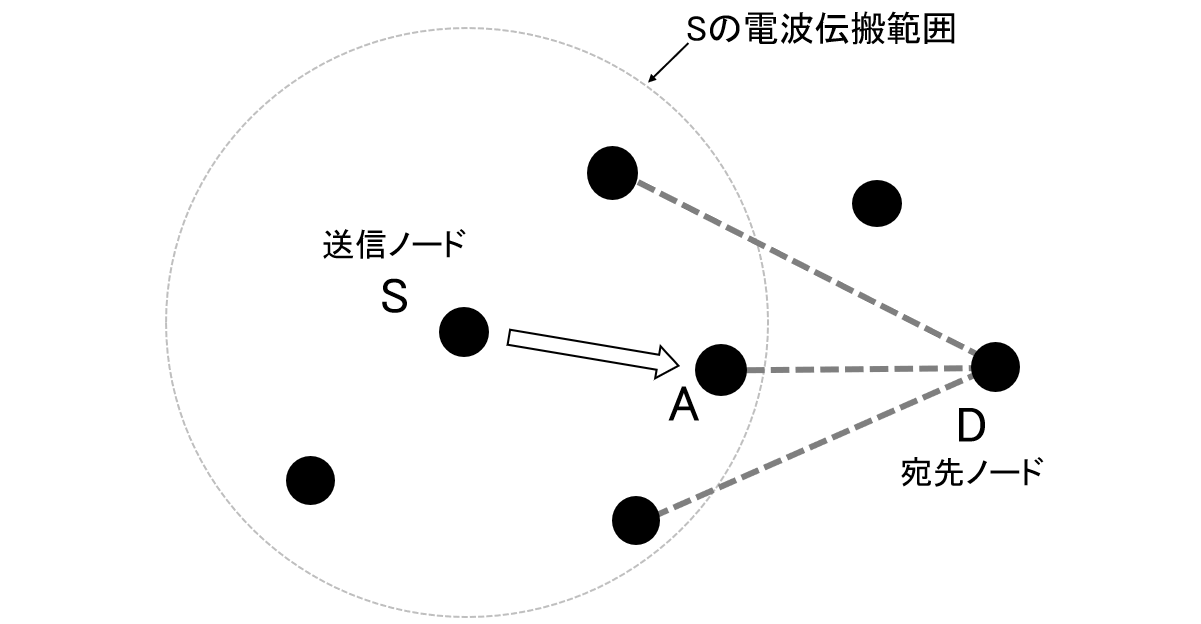
\includegraphics[scale=0.7]{figures/greedy.png}
  \caption{Greedy Forwarding}
  \label{fig:greedy}
\end{figure}

Greedy Forwardingには\textbf{局所最大問題}が存在している. 
局所最大問題とは, 図\ref{fig:local}のように, 送信ノード$S$の電波伝搬範囲内に
宛先ノード$D$が存在しない, かつ, 送信ノード$S$が自身の
電波伝搬範囲内で宛先ノード$D$に最も近い場合, 選択できる
ネクストホップが存在しなくなるという問題である.

\begin{figure}
  \centering
  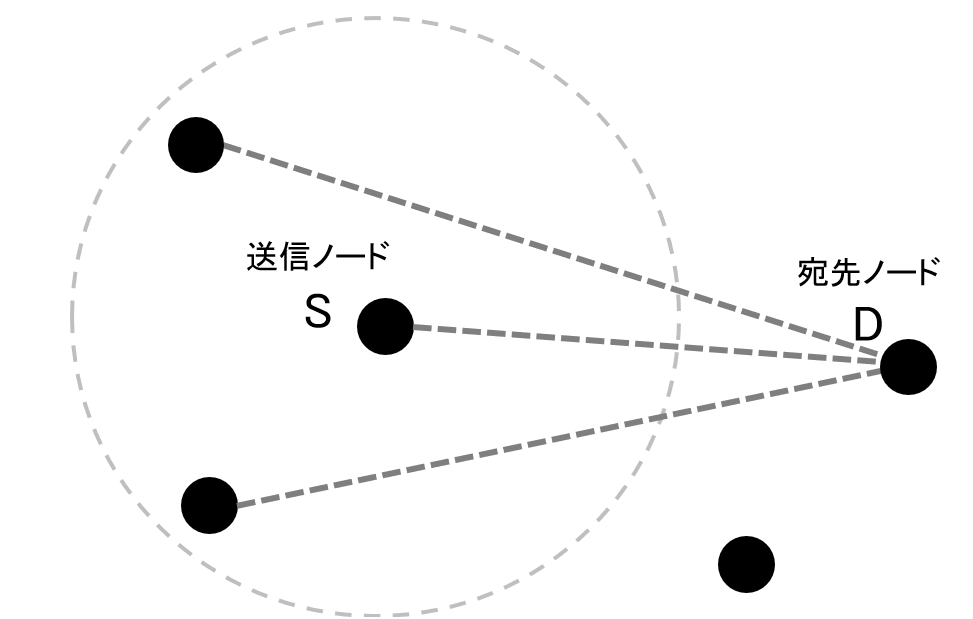
\includegraphics[scale=0.6]{figures/local.png}
  \caption{局所最大問題}
  \label{fig:local}
\end{figure}
